%!TEX root = main.tex

\subsection{Introduction}

\textbf{Problem}: Given a formal grammar G (CFG) and a sentence s, build a parse tree of s according to G. There may be no solution or many solutions (ambiguity). Context-free means that any rules used to replace the left hand side can be used anywhere in a parse tree.

\textbf{Parsing} is the search among all possible parse trees that can be generated from S for the one generating the observed sentence s. The search space can be explored \textbf{bottom-up} or \textbf{top-down}.
\\ 
\noindent
\begin{minipage}{.5\textwidth}
	\centering
	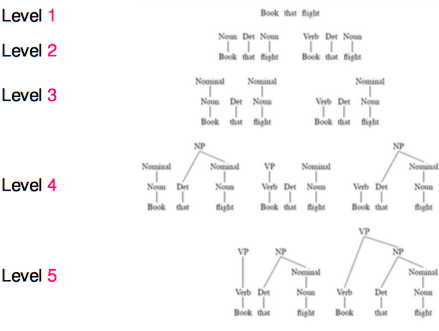
\includegraphics[scale=0.4]{images/43_bottom-up.png}
 	\captionof{figure}{Bottom-up. Never wastes time exploring tree that cannot result is an S.}
\end{minipage}%
\begin{minipage}{.5\textwidth}
	\centering
	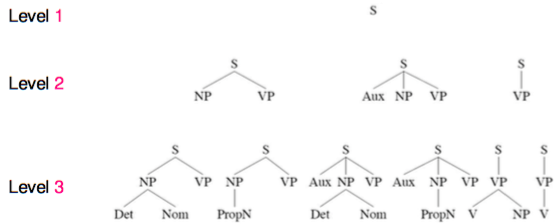
\includegraphics[scale=0.4]{images/44_top-down.png}
 	\captionof{figure}{Top-down. Never wastes time on trees that are not consistent with the input.}
\end{minipage}

Due to ambiguity, in the worst case, the number of parse trees is exponential to the sentence length.

\subsection{CYK Algorithm}

Before using the algorithm, we need to change the grammar in Chomsky Normal Form.

\begin{figure}[htp]
	\centering
	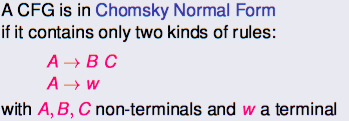
\includegraphics[scale=0.5]{images/45_chomsky.png}
 	\caption{CNF.}
\end{figure}

\begin{figure}[htp]
	\centering
	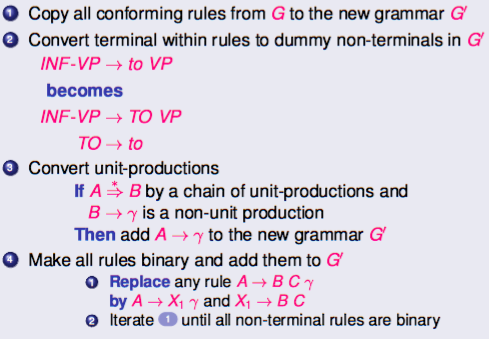
\includegraphics[scale=0.5]{images/46_conversion.png}
 	\caption{Conversion algorithm.}
\end{figure}

\begin{figure}[H]
	\centering
	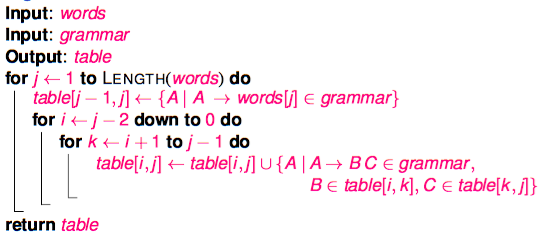
\includegraphics[scale=0.6]{images/47_cyk.png}
 	\caption{CYK algorithm. The sentence is accepted if S in $table[0,N]$. Backpointers. Bottum-up. $O(n^3)$.}
\end{figure}

\noindent
\begin{minipage}{.5\textwidth}
	\centering
	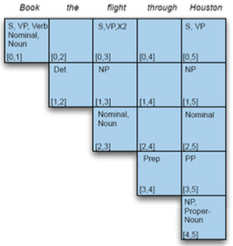
\includegraphics[scale=0.6]{images/48_table.png}
 	\captionof{figure}{Example.}
\end{minipage}%
\begin{minipage}{.5\textwidth}
	\centering
	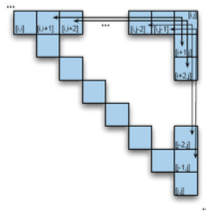
\includegraphics[scale=0.6]{images/49_order.png}
 	\captionof{figure}{Order.}
\end{minipage}


\subsection{Probabilistic CFG and probabilistic parsing}

\textbf{Problem}: Given a PCFG G and a sentence S, compute a most likely parse tree.

\begin{figure}[htp]
	\centering
	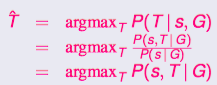
\includegraphics[scale=0.6]{images/54_prob.png}
 	\caption{Disambiguation rule.}
\end{figure}

Solve the exponential blow-up issue by computing most likely parse tree.

\begin{figure}[H]
	\centering
	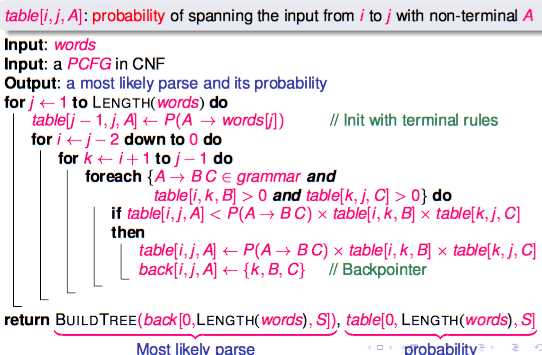
\includegraphics[scale=0.6]{images/55_prob.png}
 	\caption{Probabilistic CYK.}
\end{figure}

\subsubsection{Learning rule probabilities from a Treebank}

\begin{figure}[H]
	\centering
	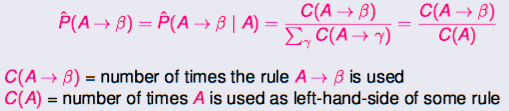
\includegraphics[scale=0.5]{images/56_learning.png}
 	\caption{Rule probability estimate. Smoothing may be used. Unsupervised learning possible: Inside-Outside algorithm.}
\end{figure}

\subsection{Earley Algorithm}

\begin{figure}[htp]
	\centering
	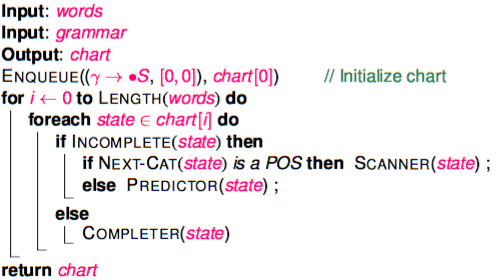
\includegraphics[scale=0.6]{images/50_earley.png}
 	\caption{Earley algorithm. Top-down. No need for CNF. A state $S \rightarrow \alpha \bullet , [0,N]$ in $chart[N]$ denotes a successful parse. $O(n^3)$. }
\end{figure}

\begin{figure}[htp]
	\centering
	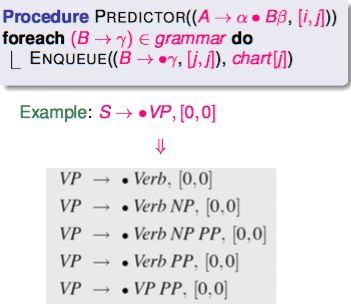
\includegraphics[scale=0.5]{images/51_predictor.png}
 	\caption{Predictor.}
\end{figure}

\begin{figure}[htp]
	\centering
	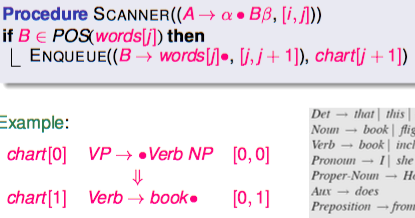
\includegraphics[scale=0.5]{images/52_scanner.png}
 	\caption{Scanner.}
\end{figure}

\begin{figure}[htp]
	\centering
	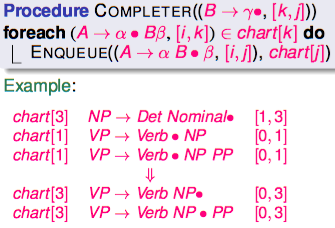
\includegraphics[scale=0.5]{images/53_completer.png}
 	\caption{Completer.}
\end{figure}

\subsection{Partial parsing}

A style of partial parsing is \textbf{chunking}: a simple bracketing without hierarchical structure. 

\subsubsection{Algorithms}

\begin{itemize}
	\item HMMs;
	\item Local classifier from selected features;
	\item Iterated chunking based on a hierarchy of chunk tag offers an approximation to full parsing.
\end{itemize}

\subsubsection{Chunking system evaluation}

\begin{figure}[htp]
	\centering
	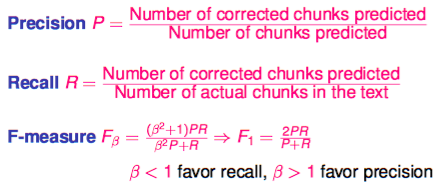
\includegraphics[scale=0.6]{images/57_eval.png}
 	\caption{Evaluation. State of art is 92\% $F_1$.}
\end{figure}